\documentclass[../report.tex]{subfiles}
\begin{document}

\section{Background} \label{sec:background}
Theory required to understand the design and choices in the report will be described in this section.

\subsection{Block Random Access Memory} \label{subsec:background_bram}
\begin{wrapfigure}{R}{0.5\textwidth}
    \centering
    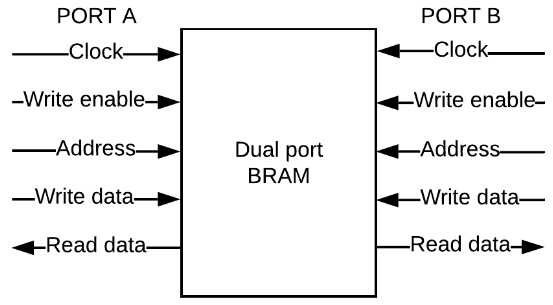
\includegraphics[width=0.45\textwidth]{figures/background/dual_port_bram.png}
    \captionsetup{width=0.45\textwidth}
    \caption{Illustration of the dual-port BRAN}
    \label{fig:simple_bram}
\end{wrapfigure}
One way to make a communication between the processor system, PS, and the programmable logic, PL, on the PYNQ Z2 board is through BRAM. BRAM is located on the FPGA and is used to store data and has a fixed size width and depth. The width of the BRAM dictates the length of a word and the depth dictates the number of words that can be stored. BRAM is synchronized via a clock signal. In order to get the correct data out of the BRAM, an address is used to point at the data location. Furthermore, a write enable pin is used to dictate whether to write or read. A simple model of BRAM in dual-port configuration is illustrated in \autoref{fig:simple_bram}.

\subsection{Analog to Digital Converter} \label{subsec:background_adc}
\begin{wrapfigure}{R}{0.5\textwidth}
    \centering
    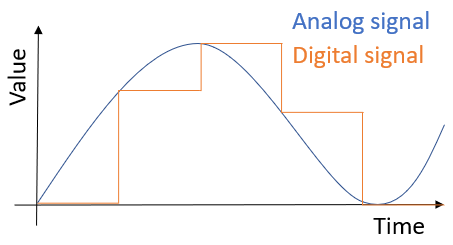
\includegraphics[width=0.45\textwidth]{figures/background/adc.png}
    \captionsetup{width=0.45\textwidth}
    \caption{Illustration of analog to digital convertion.}
    \label{fig:adc}
\end{wrapfigure}
To convert an analog signal to a digital signal an ADC, is used. The ADC converts the analog input periodically, thus the digital signal is a discretization of the analog signal. At each sampling time the ADC samples the analog signal value as a discrete value. An illustration can be seen in \autoref{fig:adc}, in which the digital signal measures the analog signal value and hold its until a new measurement is done.

\subsection{Pulse-Width Modulation}
PWM is a technique to control the average voltage applied to a component or system. This can be used to control a charging circuit which charges batteries since it would enable control of applied voltage and current to a battery.

A PWM signal is generated by usage of a timer, which is visualized in \autoref{fig:pwm:figure}.

\begin{figure}[H]
    \centering
    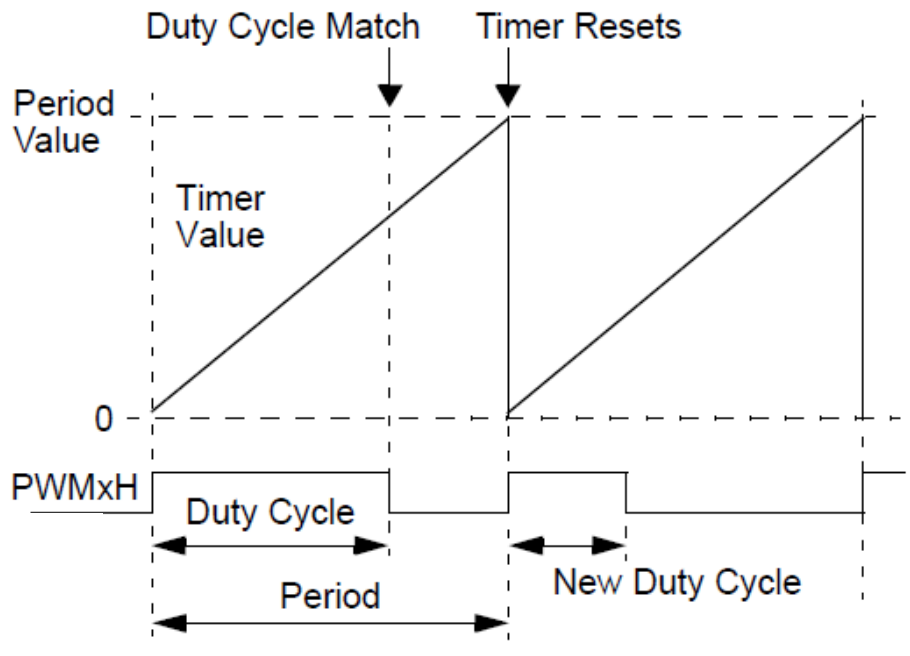
\includegraphics[width=0.5\textwidth]{figures/pwm/pwm_fig.png}
    \captionsetup{width=0.75\textwidth}
    \caption{Visualization of a PWM signal with a timer. Figure is from lecture slides by Emad Samuel Malki Ebeid.}
    \label{fig:pwm:figure}
\end{figure}

The duty cycle is the ratio of high output signal to low output signal. The duty cycle can be controlled by changing the threshold used to generate the PWM signal.

\subsection{Buck Converter}
Applying the PWM signal described above directly to a battery would probably damage the battery depending on the source voltage. Without the usage of circuits like buck converters, the charging circuit would either damage the battery during recharging or it would lose flexibility with respect to charging multiple kinds of batteries.

\begin{figure}[H]
    \centering
    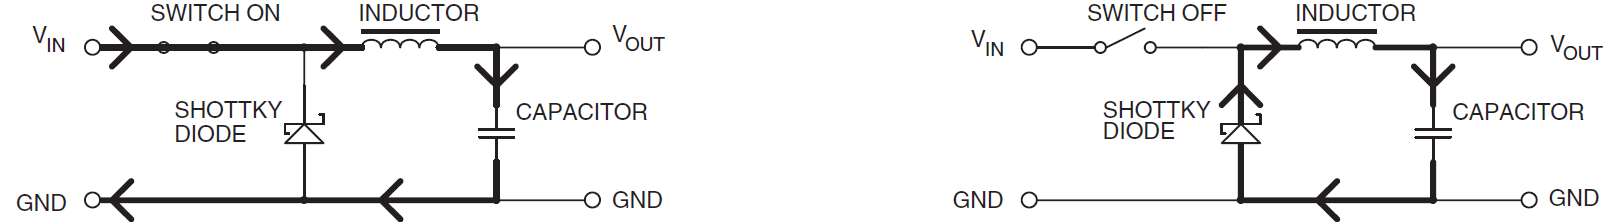
\includegraphics[width=1\textwidth]{figures/buck_converter_principle.png}
    \caption{Buck converter switching principle \cite{avr450}.}
    \label{fig:buck:principle}
\end{figure}

The principle of using a buck circuit with a PWM input controlling a switch is shown in \autoref{fig:buck:principle}. When the switch is closed the capacitor and inductor is charged when the switch opens the inductor will maintain the current by inducing a voltage.

The effect of the buck circuit is visualized in \autoref{fig:buck:graph}.

\begin{figure}[H]
    \centering
         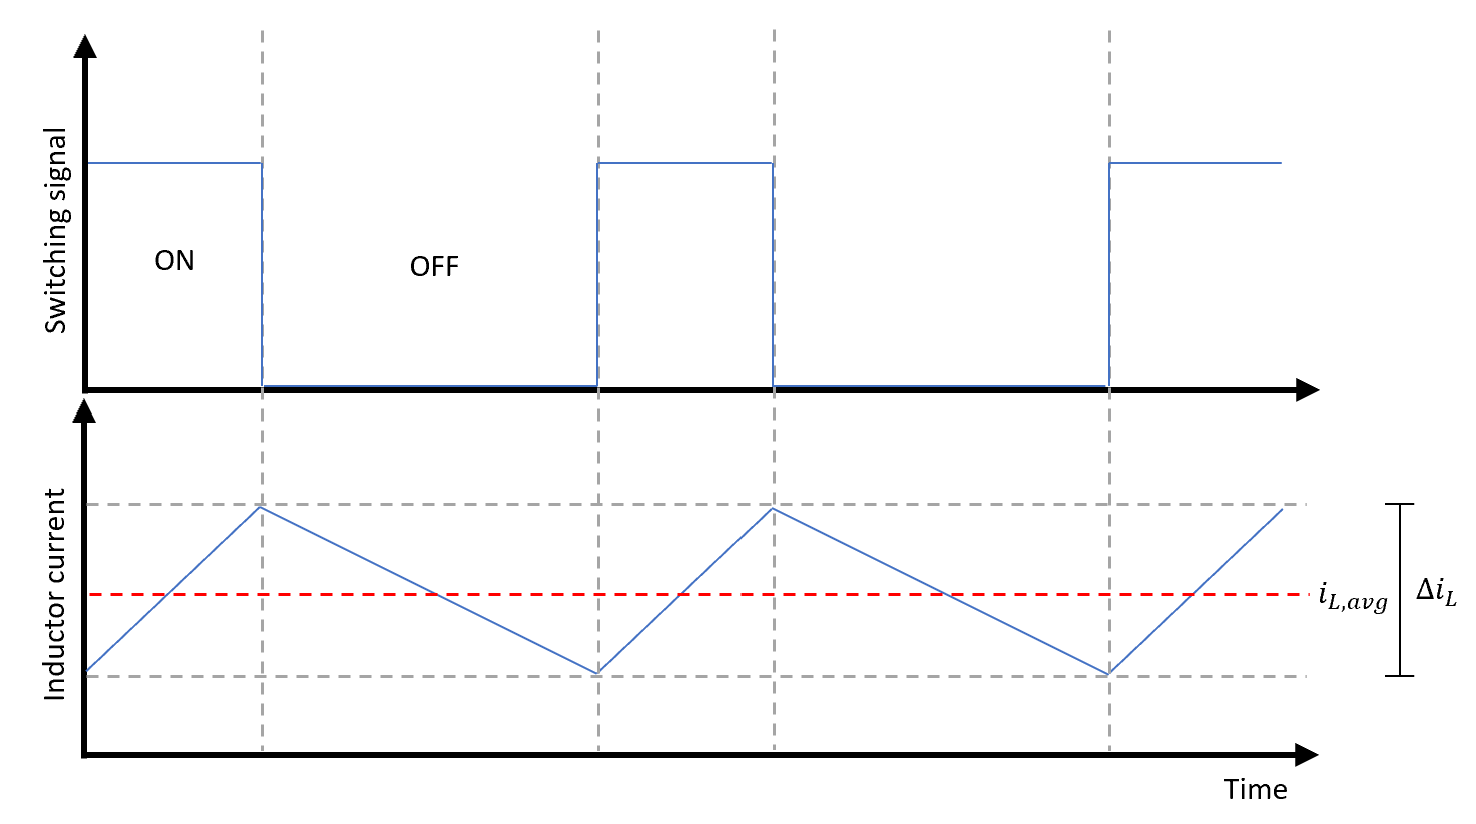
\includegraphics[width=0.90\textwidth]{figures/circuit/buck_graph.png}
     \caption{Visualization of the current looping in the buck circuit and the switching input.}
     \label{fig:buck:graph}
\end{figure}

It is seen that the Buck circuit tries to maintain the current when the PWM signal is in the off state, this is also the case for the voltage. The buck circuit will be designed based on the ripple $\Delta i_L$ and the voltage ripple $\Delta V_C$, which is not shown in \autoref{fig:buck:graph}.

\end{document}